
The pdf of $Z(=X+Y)$ will be convolution of pdf of $X$ and pdf of $Y$ as shown below.
\begin{align}
f_{x}( x)\times f_{y}(y)=f_{z}(z)
\end{align}
\tikzset{every picture/.style={line width=0.5pt}} %set default line width to 0.75pt        
\begin{tikzpicture}[x=0.45pt,y=0.5pt,yscale=-1,xscale=1]
%uncomment if require: \path (0,300); %set diagram left start at 0, and has height of 300
%Straight Lines [id:da7994322016020907] 
\draw [line width=0.75]    (65.3,280.6) -- (580.3,280.6) ;
%Straight Lines [id:da6298726397789813] 
\draw [line width=0.75]    (321.8,68.4) -- (322.8,280.6) ;
%Shape: Right Angle [id:dp8023791863547924] 
\draw  [color={rgb, 255:red, 0; green, 0; blue, 0 }  ,draw opacity=1 ][line width=1.5]  (254.8,168.6) -- (389.8,168.6) -- (389.8,279) ;
%Straight Lines [id:da07001326664875096] 
\draw [line width=1.5]    (254.8,168.6) -- (254.8,279) ;
% Text Node
\draw (403,152.4) node [anchor=north west][inner sep=0.75pt]    {$\dfrac{1}{2}$};
% Text Node
\draw (240,285.4) node [anchor=north west][inner sep=0.75pt]    {$-1$};
% Text Node
\draw (385,282.4) node [anchor=north west][inner sep=0.75pt]    {$1$};
% Text Node
\draw (318,283.4) node [anchor=north west][inner sep=0.75pt]    {$0$};
% Text Node
\draw (303,44.4) node [anchor=north west][inner sep=0.75pt]    {$f_{x}( x)$};
% Text Node
\draw (590,269.4) node [anchor=north west][inner sep=0.75pt]    {$x$};
\end{tikzpicture}
\tikzset{every picture/.style={line width=0.5pt}} %set default line width to 0.75pt        
\begin{tikzpicture}[x=0.45pt,y=0.5pt,yscale=-1,xscale=1]
%uncomment if require: \path (0,300); %set diagram left start at 0, and has height of 300
%Straight Lines [id:da7994322016020907] 
\draw [line width=0.75]    (65.3,280.6) -- (580.3,280.6) ;
%Straight Lines [id:da6298726397789813] 
\draw [line width=0.75]    (321.8,68.4) -- (322.8,280.6) ;
%Shape: Right Angle [id:dp8023791863547924] 
\draw  [color={rgb, 255:red, 0; green, 0; blue, 0 }  ,draw opacity=1 ][line width=1.5]  (267.8,168.6) -- (389.8,168.6) -- (389.8,279) ;
%Straight Lines [id:da07001326664875096] 
\draw [line width=1.5]    (267.8,168.6) -- (189.8,169.4) -- (189.8,280) ;
% Text Node
\draw (403,152.4) node [anchor=north west][inner sep=0.75pt]    {$\dfrac{1}{3}$};
% Text Node
\draw (240,282.4) node [anchor=north west][inner sep=0.75pt]    {$-1$};
% Text Node
\draw (385,282.4) node [anchor=north west][inner sep=0.75pt]    {$1$};
% Text Node
\draw (318,283.4) node [anchor=north west][inner sep=0.75pt]    {$0$};
% Text Node
\draw (303,44.4) node [anchor=north west][inner sep=0.75pt]    {$f_{y}( y)$};
% Text Node
\draw (590,269.4) node [anchor=north west][inner sep=0.75pt]    {$y$};
% Text Node
\draw (175,280.4) node [anchor=north west][inner sep=0.75pt]    {$-2$};
\end{tikzpicture}
\tikzset{every picture/.style={line width=0.5pt}} %set default line width to 0.75pt        
\begin{tikzpicture}[x=0.45pt,y=0.5pt,yscale=-1,xscale=1]
%uncomment if require: \path (0,300); %set diagram left start at 0, and has height of 300
%Straight Lines [id:da7994322016020907] 
\draw [line width=0.75]    (65.3,280.6) -- (580.3,280.6) ;
%Straight Lines [id:da6298726397789813] 
\draw [line width=0.75]    (321.8,68.4) -- (322.8,280.6) ;
%Straight Lines [id:da3048610517318646] 
\draw [line width=1.5]    (249.8,174.8) -- (322.3,174.5) ;
%Straight Lines [id:da21348606992409946] 
\draw [line width=1.5]    (249.8,174.8) -- (126.8,280.8) ;
%Straight Lines [id:da9537386999126634] 
\draw [line width=1.5]    (322.3,174.5) -- (460.8,279.8) ;
%Straight Lines [id:da7472472432945507] 
\draw  [dash pattern={on 0.84pt off 2.51pt}]  (391.55,227.15) -- (188.3,227.8) ;
%Straight Lines [id:da7478392311577124] 
\draw  [dash pattern={on 0.84pt off 2.51pt}]  (188,281) -- (188.3,227.8) ;
%Straight Lines [id:da11363593871174427] 
\draw  [dash pattern={on 0.84pt off 2.51pt}]  (253.8,278) -- (254.8,228) ;
%Straight Lines [id:da30914849700103675] 
\draw  [dash pattern={on 0.84pt off 2.51pt}]  (390.8,278) -- (391.55,227.15) ;
% Text Node
\draw (350,153.4) node [anchor=north west][inner sep=0.75pt]    {$\dfrac{1}{3}$};
% Text Node
\draw (241,282.4) node [anchor=north west][inner sep=0.75pt]    {$-1$};
% Text Node
\draw (385,282.4) node [anchor=north west][inner sep=0.75pt]    {$1$};
% Text Node
\draw (318,283.4) node [anchor=north west][inner sep=0.75pt]    {$0$};
% Text Node
\draw (271,50.4) node [anchor=north west][inner sep=0.75pt]    {$f_{Z}( z) =f_{x}( \ x) \times \ f_{y} y)$};
% Text Node
\draw (175,280.4) node [anchor=north west][inner sep=0.75pt]    {$-2$};
% Text Node
\draw (114,282.4) node [anchor=north west][inner sep=0.75pt]    {$-3$};
% Text Node
\draw (455,282.4) node [anchor=north west][inner sep=0.75pt]    {$2$};
% Text Node
\draw (586,271.4) node [anchor=north west][inner sep=0.75pt]    {$z$};
% Text Node
\draw (415,198.4) node [anchor=north west][inner sep=0.75pt]    {$\dfrac{1}{6}$};
\end{tikzpicture}
Now
\begin{align}
\pr{Z \leq z} &=\int_{-\infty}^{z} f_{Z}(z) d z \\
\pr{Z \leq-2} &=\int_{-\infty}^{-2} f_{Z}(z) d z \\
&=\text {Area }[z \leq-2] \\
&=\frac{1}{2} \times \frac{1}{6} \times 1=\frac{1}{12}
\end{align}
Hence $(\mathrm{D})$ is correct option.